\documentclass[a4paper,10pt]{article}

\usepackage[utf8]{inputenc}
\usepackage{amsmath, amssymb, hyperref, multirow, dot2texi}

\usepackage{tikz}
\usetikzlibrary{shapes, arrows}

% Title Page
\title{}
\author{}

\parskip = 8pt
\setlength{\parindent}{0pt}

\begin{document}

\section{Introduction} % Problem Formulation

In recent years, several \cite{sdf} successes have been booked for applying semantic analysis on user comments of movies.
In this report we use those same techniques, but apply them to plot summaries of movies to try and estimate the score these movies are rated with on the popular online movie database IMDb.
These user-written texts roughly describe what happens in a particular movie and may therefore be an indication of the score, which is also calculated from user submitted data.

This project is part of the Natural Language Processing course of the UvA from Fall 2014.

\section{Models}
In this section we describe our extended topic based model.

The traditional topic based model used in LDA can be seen in Figure~\ref{fig:LDA}.
In it, we can see that the topic distribution from which a document is drawn is parametrized by $\theta_d$, which is determined according to some distribution of hyperparameter $\alpha$.

\begin{figure}[ht!]
  \centering
  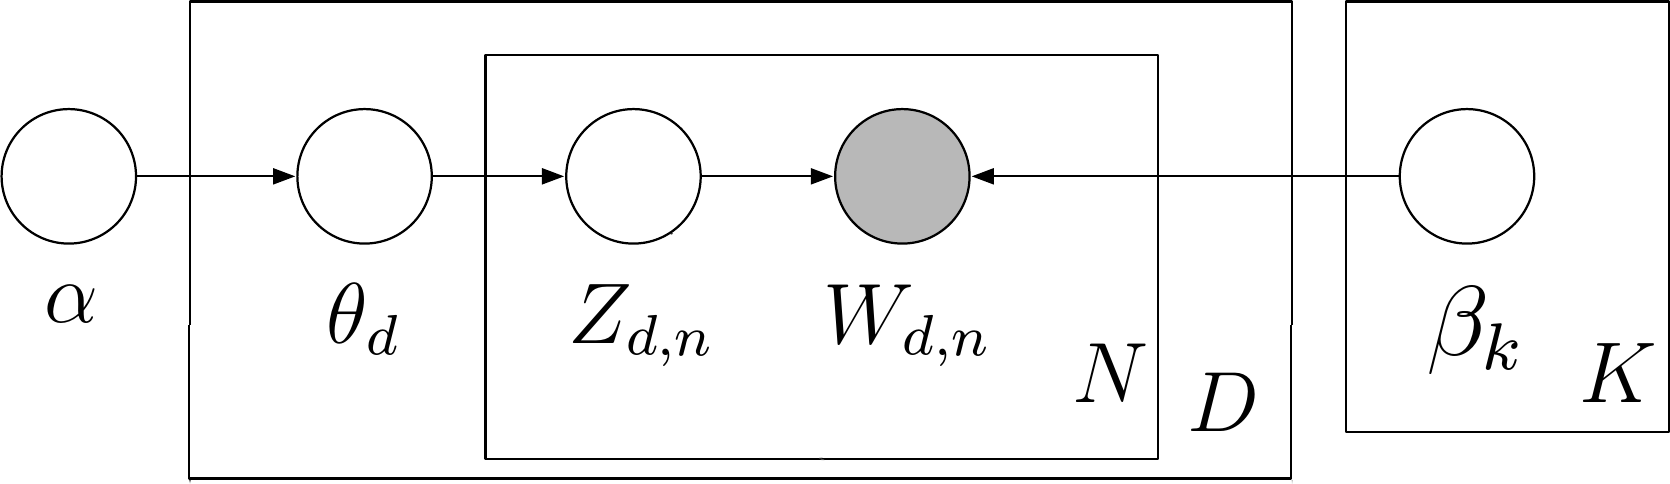
\includegraphics[width=\textwidth]{LDA.png}
  \label{fig:LDA}
  \caption{A graphical representation of traditional LDA model.}
\end{figure}

\begin{figure}[ht!]
  \centering
  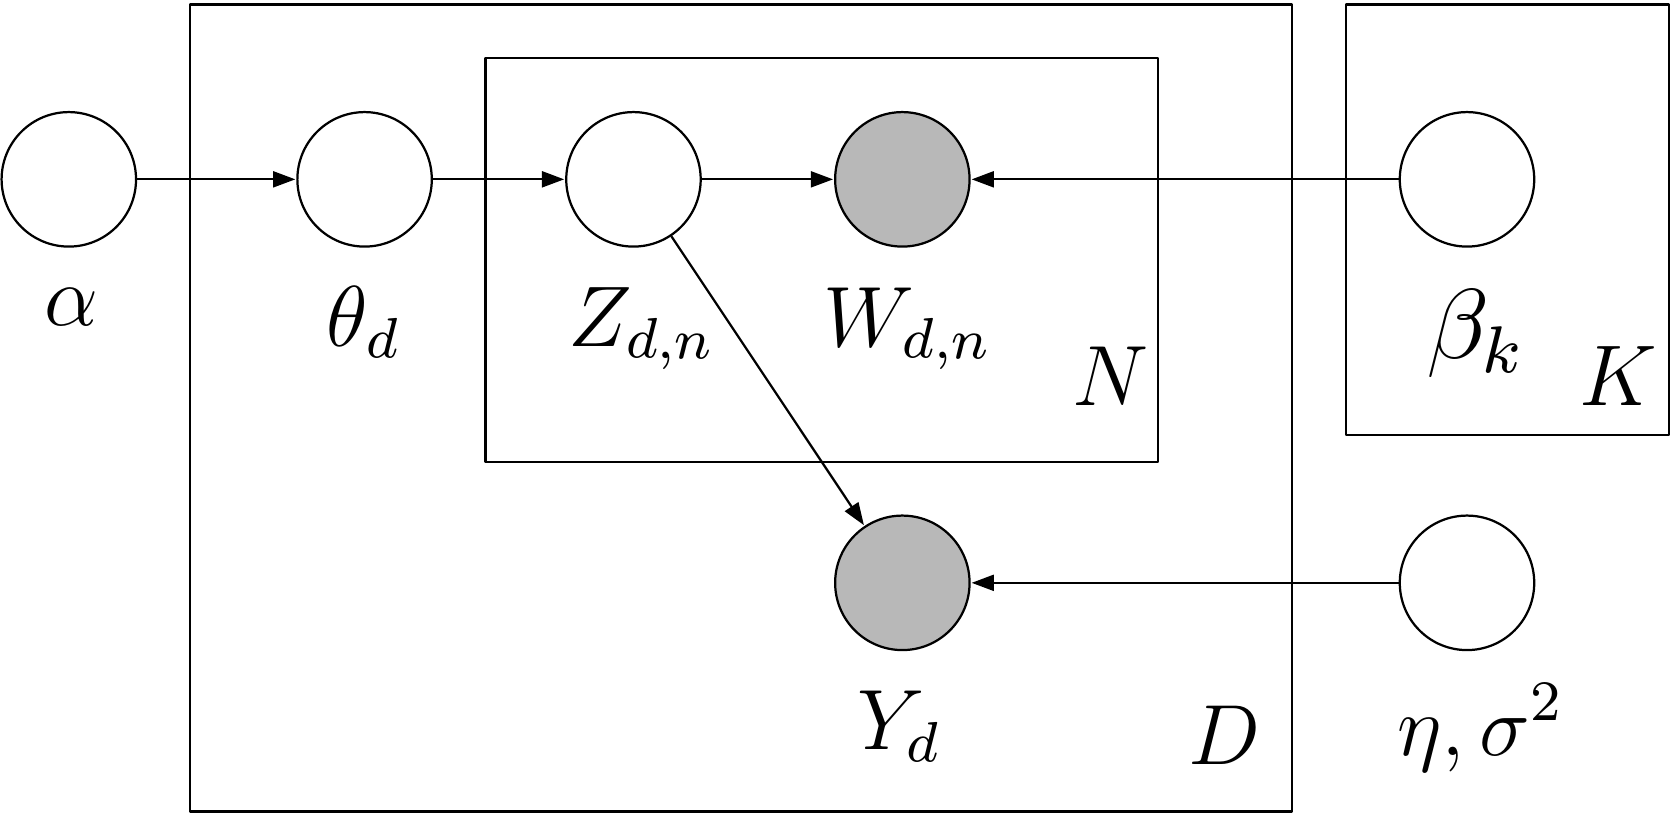
\includegraphics[width=\textwidth]{SLDA.png}
  \label{fig:SLDA}
  \caption{A graphical representation of our modified LDA model.}
\end{figure}

\section{Approach}

\section{Dataset}

\section{Experiments}

\section{Results}

\section{Discussion}



Collapsed Segmented LDA (CSLDA):

$$ p(S, Z, W | \alpha, \beta, \eta, \sigma) = \left[ \prod_k \frac{\Gamma(W \beta)}{\Gamma(\beta)^W \cdot \Gamma(N_k + W \beta)} \prod_w \Gamma(N_{kw} + \beta) \right] $$
$$ \times \left[ \prod_d \mathcal{N}\left(s_d\, \left|\, \eta^T \cdot \frac{N_{dk}}{N_d}, \sigma\right. \right) \frac{\Gamma(K \alpha)}{\Gamma(\alpha)^K \cdot \Gamma(N_d + K \alpha)} \prod_k \Gamma(N_{dk} + \alpha) \right] $$

Where we used $ \frac{N_{dk}}{N_d} \equiv \bar{Z_d} $

$$ \log p(S, Z, W | \alpha, \beta, \eta, \sigma) = $$
$$ \left[ \sum_k \log \Gamma(W \beta) - W \log \Gamma(\beta) - \log \Gamma(N_k + W \beta) + \sum_w \log \Gamma(N_{kw} + \beta) \right] $$
$$ + \left[ \sum_d \underbrace{- \log \sigma - \frac{1}{2} \log(2 \pi) - \frac{\left(s_d - \eta^T \cdot \frac{N_{dk}}{N_d}\right)^2}{2 \sigma^2}}_{\text{Normal distribution}} + \right. $$
$$ \left. \log \Gamma(K \alpha) - K \log \Gamma(\alpha) - \log \Gamma(N_d + K \alpha) + \sum_k \log \Gamma(N_{dk} + \alpha) \right] $$

Maximum a posteriori (MAP) estimate for the $\eta$ hyperparameter:

$$ \nabla_{\eta_k} \log p(S, Z, W | \alpha, \beta, \eta, \sigma) = \sum_d \frac{ \frac{N_{dk}}{N_d} \left( s_d - \eta^T \frac{N_{d\cdot}}{N_d}\right) }{\sigma^2} = $$
$$ = \sum_d \frac{s_d \frac{N_{dk}}{N_d} }{\sigma^2} - \sum_d \frac{ \frac{N_{dk}}{N_d} \left( \eta^T \frac{N_{d\cdot}}{N_d} \right) }{\sigma^2} = 0 $$
$$ \Rightarrow \sum_d s_d \frac{N_{dk}}{N_d} = \sum_d \frac{N_{dk}}{N_d} \left( \sum_{k'} \eta_{k'} \frac{N_{dk'}}{N_d} \right) = \sum_d \frac{N_{dk}}{N_d} \left( \eta_k \frac{N_{dk}}{N_d} + \sum_{k' \ne k} \eta_{k'} \frac{N_{dk'}}{N_d} \right) $$
$$ \Rightarrow \sum_d s_d \frac{N_{dk}}{N_d} = \eta_k \sum_d \left( \frac{N_{dk}}{N_d}  \right)^2 + \sum_d \left( \frac{N_{dk}}{N_d} \sum_{k' \ne k} \eta_{k'} \frac{N_{dk'}}{N_d} \right) $$
$$ \Rightarrow \sum_d \left( s_d \frac{N_{dk}}{N_d} - \frac{N_{dk}}{N_d} \sum_{k' \ne k} \eta_{k'} \frac{N_{dk'}}{N_d} \right) = \eta_k \sum_d \left( \frac{N_{dk}}{N_d}  \right)^2 $$
$$ \Rightarrow \sum_d \frac{N_{dk}}{N_d} \left( s_d - \sum_{k' \ne k} \eta_{k'} \frac{N_{dk'}}{N_d} \right) = \eta_k \sum_d \left( \frac{N_{dk}}{N_d}  \right)^2 $$
$$ \Rightarrow \eta_k = \frac{\sum_d \frac{N_{dk}}{N_d} \left( s_d - \sum_{k' \ne k} \eta_{k'} \frac{N_{dk'}}{N_d} \right)}{\sum_d \left( \frac{N_{dk}}{N_d}  \right)^2} $$

Trying to apply the previous formula as an update rule for $\eta$ does not converge. Instead, the following update can be used:

$$ \eta_k^{new} \leftarrow (1 - \gamma) \eta_k^{old} + \gamma \frac{\sum_d \frac{N_{dk}}{N_d} \left( s_d - \sum_{k' \ne k} \eta_{k'} \frac{N_{dk'}}{N_d} \right)}{\sum_d \left( \frac{N_{dk}}{N_d}  \right)^2 + \epsilon}$$

With $1 \gg \gamma > 0$ in order for the previous series to converge and $1 \gg \epsilon > 0$ is a smoothing constant.

Gibbs sampler:

$$ p(z_{di} = k | Z^{\backslash i}, S, W, \alpha, \beta, \eta, \sigma) \propto p(z_{di} = k, Z_{-i}, S, W, \alpha, \beta, \eta, \sigma) $$
$$ \propto \left[ \prod_{k'} \frac{\prod_w \Gamma(N_{{k'}w}^{\backslash i} + 1(k' = k \wedge w = w_{di}) + \beta)}{\Gamma(N_{k'}^{\backslash i} + 1(k' = k) + W \beta)} \right] \times $$
$$ \mathcal{N}\left(s_d\, \left|\, \eta^T \cdot \frac{N_{d{k'}}^{\backslash i} + 1(k' = k)}{N_d}, \sigma\right. \right) \prod_{k'} \Gamma(N_{d{k'}}^{\backslash i} + 1(k' = k) + \alpha) $$


\end{document}          
